\documentclass[a4paper]{article}
\usepackage[a4paper,top=2cm,bottom=2cm,left=0.5cm,right=0.5cm,marginparwidth=1.75cm]{geometry}
\usepackage[]{graphicx}
\usepackage[]{wrapfig}
\usepackage[T2A]{fontenc}
\usepackage[utf8]{inputenc}
\usepackage[english, russian]{babel}
\usepackage[]{amsmath,amsfonts,amssymb,amsthm,mathtools}
\usepackage[]{wasysym}
\usepackage[]{float}
\usepackage{multicol}
\usepackage{mathtext}
\usepackage{amsmath}
\usepackage{amsfonts}
\usepackage{indentfirst}
\usepackage{longtable}
\usepackage{natbib}
\usepackage{mathrsfs}
\title{Исследование неизвестной на момент заголовка функции}
\date{\today}
\begin{document}
\maketitle
\section{Введение в проблему}
На операционном столе сегодня находится следующая функция:\\
$f(x) = x*12^{x}$\\
После некоторых очевиднейших преобразований получаем :\\
$f(x) = x*12^{x}$\\
\section{Нахождение первой производной}
Найдем $f\prime(x)$ :\\Если бы вы посещали вуз, вы бы знали, что:\\
$(x)\prime *12^{x}+x*(12^{x}$\\
И.Р. Дединский всегда говорил, что:\\
$\frac{1}{x}*(x)\prime *12^{x}+x*(12^{x}$\\
Очевидно, что:\\
$\frac{1}{x}*1*x^{0}*12^{x}+x*12*12^{x}*(x)\prime $\\
Имеем $f\prime(x) = x^{-1}*12^{x}+x*12*12^{x}$\\
\section{Нахождение второй производной}
$f\prime\prime(x) = (x^{-1}*12^{x}+x*12*12^{x})\prime $\\ 
Ладно:\\
$(x^{-1}*12^{x})\prime +(x*12*12^{x})\prime $\\
На пятой лекции Знаменской доказывалось, что:\\
$-1*x^{-2}*12^{x}+x^{-1}*12*12^{x}*(x)\prime +(x*12*12^{x})\prime $\\
Ничто не точно, разве что:\\
$-1*x^{-2}*12^{x}+x^{-1}*12*12^{x}*1*x^{0}+\frac{1}{x}*1*x^{0}*12*12^{x}+x*(\frac{1}{12}*(12)\prime *12^{x}+12*(12^{x})$\\
Имеем $f\prime\prime(x) = -1*x^{-2}*12^{x}+x^{-1}*12*12^{x}+x^{-1}*12*12^{x}+x*12*12*12^{x}$\\
\section{Найдем первую и вторую производную в точке, а также саму функцию}
$f(2) = 99.8132$\\
$f\prime(2) = 320.026 $\\
И вторую производную: \\ 
$f(2)\prime\prime = 938.149$ \\
\section{График}
На данном графике в районе $\pm 2$ от заданной точки указаны: \\
Красный - сама функция \\
Зеленый - первая производная \\
Синий - вторая производная \\
\begin{figure}[H]
\centering
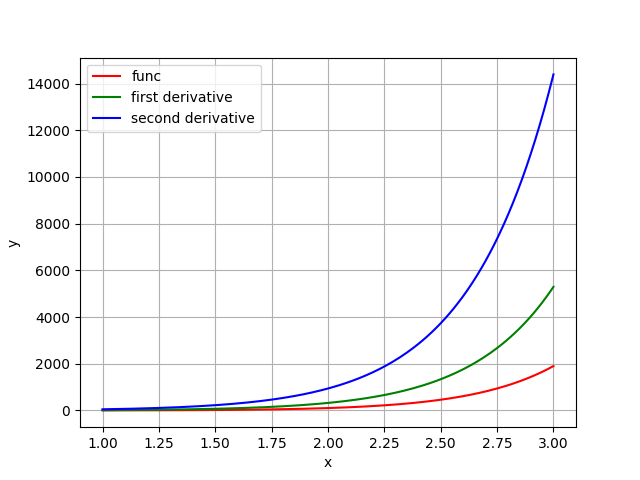
\includegraphics{graph.png}
\end{figure}\section{Тэйлор в точке до o($x^7$)}
Далее мы неиронично разложим функцию в ряд тэйлора в точке $x0 = 2$: \\
$f(x) = 99.8132 + \frac{320.026}{1}(x-2)^{1} + \frac{938.149}{2}(x-2)^{2} + \frac{2632.88}{6}(x-2)^{3} + \frac{7194.71}{24}(x-2)^{4} + \frac{19318.9}{120}(x-2)^{5} + \frac{51225.4}{720}(x-2)^{6} + \frac{134582}{5040}(x-2)^{7} + o(x^7)$
\end{document}